%==============================================================================
% tento soubor pouzijte jako zaklad
% this file should be used as a base for the thesis
% Autoři / Authors: 2008 Michal Bidlo, 2016 Jaroslav Dytrych
% Kontakt pro dotazy a připomínky: dytrych@fit.vutbr.cz
% Contact for questions and comments: dytrych@fit.vutbr.cz
%==============================================================================
% kodovaní: UTF-8 (zmena prikazem iconv, recode nebo cstocs)
% encoding: UTF-8 (you can change it by command iconv, recode or cstocs)
%------------------------------------------------------------------------------
% zpracování / processing: make, make pdf, make clean
%==============================================================================
% Soubory, které je nutné upravit: / Files which have to be edited:
%   projekt-20-literatura-bibliography.bib - literatura / bibliography
%   projekt-01-kapitoly-chapters.tex - obsah práce / the thesis content
%   projekt-30-prilohy-appendices.tex - přílohy / appendices
%==============================================================================
\documentclass[english]{fitthesis} % bez zadání - pro začátek práce, aby nebyl
% problém s překladem \documentclass[english]{fitthesis} % without assignment - for the work start to avoid compilation problem
%\documentclass[zadani]{fitthesis} % odevzdani do wisu - odkazy jsou barevné
%\documentclass[english,zadani]{fitthesis} % for submission to the IS FIT - links are color
%\documentclass[zadani,print]{fitthesis} % pro tisk - odkazy jsou černé
%\documentclass[zadani,cprint]{fitthesis} % pro barevný tisk - odkazy jsou černé, znak VUT barevný
%\documentclass[english,zadani,print]{fitthesis} % for the color print - links are black
%\documentclass[english,zadani,cprint]{fitthesis} % for the print - links are black, logo is color
% * Je-li prace psana v anglickem jazyce, je zapotrebi u tridy pouzit 
%   parametr english nasledovne:
%   If thesis is written in english, it is necessary to use 
%   parameter english as follows:
%      \documentclass[english]{fitthesis}
% * Je-li prace psana ve slovenskem jazyce, je zapotrebi u tridy pouzit 
%   parametr slovak nasledovne:
%      \documentclass[slovak]{fitthesis}

% Základní balíčky jsou dole v souboru šablony fitthesis.cls
% Basic packages are at the bottom of template file fitthesis.cls
%zde muzeme vlozit vlastni balicky / you can place own packages here

%---rm---------------
\renewcommand{\rmdefault}{lmr}%zavede Latin Modern Roman jako rm / set Latin Modern Roman as rm
%---sf---------------
\renewcommand{\sfdefault}{qhv}%zavede TeX Gyre Heros jako sf
%---tt------------
\renewcommand{\ttdefault}{lmtt}% zavede Latin Modern tt jako tt

% vypne funkci šablony, která automaticky nahrazuje uvozovky,
% aby nebyly prováděny nevhodné náhrady v popisech API apod.
% disables function of the template which replaces quotation marks
% to avoid unnecessary replacements in the API descriptions etc.
\csdoublequotesoff

% =======================================================================
% balíček "hyperref" vytváří klikací odkazy v pdf, pokud tedy použijeme pdflatex
% problém je, že balíček hyperref musí být uveden jako poslední, takže nemůže
% být v šabloně
% "hyperref" package create clickable links in pdf if you are using pdflatex.
% Problem is that this package have to be introduced as the last one so it 
% can not be placed in the template file.
\ifWis
\ifx\pdfoutput\undefined % nejedeme pod pdflatexem / we are not using pdflatex
\else
  \usepackage{color}
  \usepackage[unicode,colorlinks,hyperindex,plainpages=false,pdftex]{hyperref}
  \definecolor{links}{rgb}{0.4,0.5,0}
  \definecolor{anchors}{rgb}{1,0,0}
  \def\AnchorColor{anchors}
  \def\LinkColor{links}
  \def\pdfBorderAttrs{/Border [0 0 0] }  % bez okrajů kolem odkazů / without margins around links
  \pdfcompresslevel=9
\fi
\else % pro tisk budou odkazy, na které se dá klikat, černé / for the print clickable links will be black
\ifx\pdfoutput\undefined % nejedeme pod pdflatexem / we are not using pdflatex
\else
  \usepackage{color}
  \usepackage[unicode,colorlinks,hyperindex,plainpages=false,pdftex,urlcolor=black,linkcolor=black,citecolor=black]{hyperref}
  \definecolor{links}{rgb}{0,0,0}
  \definecolor{anchors}{rgb}{0,0,0}
  \def\AnchorColor{anchors}
  \def\LinkColor{links}
  \def\pdfBorderAttrs{/Border [0 0 0] } % bez okrajů kolem odkazů / without margins around links
  \pdfcompresslevel=9
\fi
\fi
% Řešení problému, kdy klikací odkazy na obrázky vedou za obrázek
% This solves the problems with links which leads after the picture
\usepackage[all]{hypcap}

% Informace o práci/projektu / Information about the thesis
%---------------------------------------------------------------------------
\projectinfo{
  %Prace / Thesis
  project=DP,            %typ prace BP/SP/DP/DR  / thesis type (SP = term
  % project)
  year=2017,             %rok odevzdání / year of submission
  date=\today,           %datum odevzdani / submission date
  %Nazev prace / thesis title
  title.cs={Název práce},  %nazev prace v cestine ci slovenstine (dle zadani) / thesis title in czech language (according to assignment)
  title.en={Remote API Web Reference for Java Enterprise Applications}, %nazev
  % prace v anglictine / thesis title in english Autor / Author
  author={Ondřej Krpec},   %cele jmeno a prijmeni autora / full name
  % and surname of the author
  author.name={Ondřej},   %jmeno autora (pro citaci) / author name (for
  % reference)
  author.surname={Krpec},   %prijmeni autora (pro citaci) / author surname (for
  % reference) author.title.p=Bc., %titul pred jmenem (nepovinne) / title before the name (optional)
  %author.title.a=PhD, %titul za jmenem (nepovinne) / title after the name (optional)
  %Ustav / Department
  author.title.p=Bc.,
  department=UIFS, % doplnte prislusnou zkratku dle ustavu na zadani:
  % UPSY/UIFS/UITS/UPGM                  fill in appropriate abbreviation of the department according to assignment: UPSY/UIFS/UITS/UPGM
  %Skolitel / supervisor
  supervisor=Radek Kočí, %cele jmeno a prijmeni skolitele / full name and
  % surname of the supervisor
  supervisor.name={Radek},   %jmeno skolitele (pro citaci) / supervisor name
  % (for reference)
  supervisor.surname={Kočí},   %prijmeni skolitele (pro citaci) / supervisor
  % surname (for reference)
  supervisor.title.p=Ing.,   %titul pred jmenem (nepovinne) / title before the
  % name (optional)
  supervisor.title.a={Ph.D.},    %titul za jmenem (nepovinne) / title after the name (optional)
  %Klicova slova, abstrakty, prohlaseni a podekovani je mozne definovat 
  %bud pomoci nasledujicich parametru nebo pomoci vyhrazenych maker (viz dale)
  %Keywords, abstracts, declaration and acknowledgement can be defined by following 
  %parameters or using dedicated macros (see below)
  %===========================================================================
  %Klicova slova / keywords
  %keywords.cs={Klíčová slova v českém jazyce.}, %klicova slova v ceskem ci slovenskem jazyce
  %                                              keywords in czech or slovak language
  %keywords.en={Klíčová slova v anglickém jazyce.}, %klicova slova v anglickem jazyce / keywords in english
  %Abstract
  %abstract.cs={Výtah (abstrakt) práce v českém jazyce.}, % abstrakt v ceskem ci slovenskem jazyce
  %                                                         abstract in czech or slovak language
  %abstract.en={Výtah (abstrakt) práce v anglickém jazyce.}, % abstrakt v anglickem jazyce / abstract in english
  %Prohlaseni / Declaration
  %declaration={Prohlašuji, že jsem tuto bakalářskou práci vypracoval samostatně pod vedením pana ...},
  %Podekovani (nepovinne) / Acknowledgement (optional)
  %acknowledgment={Zde je možné uvést poděkování vedoucímu práce a těm, kteří poskytli odbornou pomoc.} % nepovinne
  %acknowledgment={Here it is possible to express thanks to the supervisor and to the people which provided professional help.} % optional
}

%Abstrakt (cesky, slovensky ci anglicky) / Abstract (in czech, slovak or english)
\abstract[cs]{V~softwarovém průmyslu je kvalitní a~přístupný kód kritický pro
tvorbu moderních aplikací, a~nejlepším způsobem, jak jej zpřístupnit je pomocí
API. Nicméně nejen, že v~současné době neexistuje žádný standard pro návrh API,
ale neexistuje ani žádný standard, jak API dokumentovat. API by mělo propojovat
vývojáře a~umožnit jim snadné sdílení jejich kódu. Aby~tedy bylo užitečné,
musí pro něj existovat čistá a~čitelná dokumentace. Cílem této práce
je vývoj nástroje, který umožní nejen jednoduché a~současně propacované
zobrazení API, ale také jeho testování a~volání jednotlivých webových služeb,
které poskytuje. Práce staví na~již existujícím nástroji JRAPIDoc,
který umožňuje z~kódu automaticky vytvořit API, ale postrádá jejich kvalitní
a~jednoduchou prezentaci.} 
\abstract[en]{In~the~software industry, the~great and~accessible
code is crucial for modern businesses, and~the~best way for us to~connect
and~share it is through APIs. But not only has there been no industry standard
for designing APIs, there hasn't been an~industry standard for~documenting them.
APIs are supposed to~connect engineers and~allow for~the~sharing of~great
developments. But an~API is only valuable if it's accessible. And~for~that, it
needs clear, human and~machine readable documentation. The~aim of~the~thesis is
to~develop a~generic remote API web reference for Java Enterprise applications.
The work builds on~an~existing tool JRAPIDoc which currently lacks a~good
representation of~the~remote interfaces. Ultimately, JRAPIDoc should provide not
only a~remote API reference but also the functionality to~test and~call
the~listed web services.}

%Klicova slova (cesky, slovensky ci anglicky) / Keywords (in czech, slovak or english)
\keywords[cs]{Vzdálená~API, Webové~služby, REST, JRAPIDoc, Angular, TypeScript,
PatternFly, Red~Hat} 
\keywords[en]{Remote~API, Web~Services, REST, JRAPIDoc, Angular, TypeScript,
PatternFly, Java Enterprise Applications, Red~Hat}

%Prohlaseni (u anglicky psane prace anglicky, u slovensky psane prace slovensky)
%Declaration (for thesis in english should be in english)
\declaration{Hereby I declare that this master's thesis was prepared as an
original author's work under the supervision of Mr. Ing. Radek Kočí, Ph.D.
The supplementary information was provided by Mr. Mrg. Ivo Bek. All the relevant
information sources, which were used during preparation of this thesis, are
properly cited and included in the list of references.}

% \declaration{Hereby I declare that this bachelor's thesis was prepared as an original author’s work under the supervision of Mr. X
% The supplementary information was provided by Mr. Y
% All the relevant information sources, which were used during preparation of this thesis, are properly cited and included in the list of references.}

%Podekovani (nepovinne, nejlepe v jazyce prace) / Acknowledgement (optional, ideally in the language of the thesis
\acknowledgment{I would like to thank Mr. Mgr. Ivo Bek for his technical leading
of this Master Thesis. At the same time, I would like to thank Mr. Ing. Radek
Kočí, Ph.D., for his pedagogical leadership.}

%\acknowledgment{Here it is possible to express thanks to the supervisor and to the people which provided professional help
%(external submitter, consultant, etc.).}

% řeší první/poslední řádek odstavce na předchozí/následující stránce
% solves first/last row of the paragraph on the previous/next page
\clubpenalty=10000
\widowpenalty=10000

\begin{document}
  % Vysazeni titulnich stran / Typesetting of the title pages
  % ----------------------------------------------
  \maketitle
  % Obsah
  % ----------------------------------------------
  \setlength{\parskip}{0pt}

  {\hypersetup{hidelinks}\tableofcontents}
  
  % Seznam obrazku a tabulek (pokud prace obsahuje velke mnozstvi obrazku, tak se to hodi)
  % List of figures and list of tables (if the thesis contains a lot of pictures, it is good)
  \ifczech
    \renewcommand\listfigurename{Seznam obrázků}
  \fi
  \ifslovak
    \renewcommand\listfigurename{Zoznam obrázkov}
  \fi
  % \listoffigures
  
  \ifczech
    \renewcommand\listtablename{Seznam tabulek}
  \fi
  \ifslovak
    \renewcommand\listtablename{Zoznam tabuliek}
  \fi
  % \listoftables 

  \ifODSAZ
    \setlength{\parskip}{0.5\bigskipamount}
  \else
    \setlength{\parskip}{0pt}
  \fi

  % vynechani stranky v oboustrannem rezimu
  % Skip the page in the two-sided mode
  \iftwoside
    \cleardoublepage
  \fi

  % Text prace / Thesis text
  % ----------------------------------------------
  
% =============================================================================



\chapter{Introduction}
In~the~software industry, the~accessible and~testable code is crucial for~modern
businesses, and~the~best way for~developers to~access or~test it is through
APIs\footnote{API is an~abbreviation for~an~Application Programming Interface
which is a~set of~protocols and~tools for~building application software.}. APIs
are supposed to~connect engineers, let companies add value to~their~products
and~create an~ecosystem of~shared knowledge that allows other developers to~use
the~functions provided by~the~interfaces. To~fulfill these tasks, the~interfaces
have to~be clear, accessible and~most importantly human and~machine readable. 
However, despite their importance, there hasn't been an~industry standard
for~documentating nor~testing them.

The~thesis aims to~solve the~problem of~testing the~applications interfaces.
The~goal is to~develop an~application having an~innovative user interface
with~regard to~clarity and~simple use, aimed to~developers, even in~case
of~large interfaces. The~application will be based on~Swagger framework, which
provides a~way to~automate API reference generation. The~resulting application,
called Restty, will provide not~only way to~test single API endpoints, but
mainly the~functionality to~create extensive test cases from~the~listed web
services.

The~thesis is organized as~follows. Chapter~\ref{Preliminaries} gives
definitions needed to~follow the~thesis and~explains web services and~RESTful
APIs in~detail. Chapter~\ref{Technologies} focuses on~technologies that were
used for~development of~the~Restty application. Chapter~\ref{Design} describes
the~application's designs and~mockups, which were used to~reveal any clashing
visual elements before writing the~code. The~second to~last
Chapter covers the~development of~Restty using the~technologies listed
in~previous sections and~testing the~application using the~API from~the~Red Hat
JBoss BPM Suite application. The~last Chapter contains an~overall summary
of~the~developed solution and~final thoughts on~the~work done within the~thesis.



% =============================================================================



\chapter{Preliminaries and Definitions}
\label{Preliminaries}
This chapter will gradually introduce terms necessary to~follow the~thesis.
In~the~first section is introduced basic terminology and~established notion
of~remote interfaces and~web services. In~the~next section is provided
an~explanation of~what APIs are and~the~last section covers the~importance
of~theirs testing.



\section{Understanding the Web Services}
\label{WebServices}
A~web service is a~software system designed to~support interoperable machine
to~machine interactions over~a~network. It is a~collection of~open protocols
and~standards used for~exchanging data between applications or~systems. Software
applications written in~various programming languages and~running on~various
platforms can use web services to~exchange data over~the~networks like
the~Internet in~a~manner similar to~interprocess communication on~a~single
computer.

In~the~past, web services used mostly SOAP\footnote{Simple Object Access
Protocol is a~protocol specification for~exchanging structured information
in~the~implementation of~web services in~the~computer networks.} over~HTTP
protocol~\cite{HTTP}, allowing less costly interactions over~the~Internet.
However, in~2004 the~W3C extended the~definition of~web services
about~\uv{REST-complient} web services~\cite{W3CWebServices}, in~which
the~primary purpose of~the~web service is to~manipulate XML or~JSON
representations of~web resources using a~uniform set of~stateless operations.



\subsection{Introduction to RESTful Web Services}
The~REST, abbreviation of~Representationl State Transfer, is an~architectural
style for~networked hypermedia applications, primarily used to~build web
services. The~term was first defined in~the~year~2000 by~R.~Fielding in~his
doctoral dissertation~\cite{FieldingDissertation}. In~the~dissertation, Fielding
explained that the~REST principles were known as~the~\uv{HTTP object model}
beginning in~1994, and~were used in~designing the~HTTP~1.1 and~Uniform Resource
Identifiers~\cite{URI-RFC} standards.

The~REST architectural style constrains an~architecture to~a~\uv{client-server}
architecture and~is designed to~use a~stateless communication protocol,
typically HTTP. A~client and~a~server exchange representations of~resources
by~using standardized interface and~a~protocol. When the~client accesses
the~resource using unique URI, a~representation of~the~resource is returned.
With~each new resource representation, the~client is said to~transfer state.
The~resources are typically represented by~text, JSON or~XML, while JSON being
currently the~most popular format being used.



\subsection{Messaging}
As~mentioned in~previous section, the~RESTful web services can use any stateless
communication protocol as~a~medium of~communication between client and~a~server.
However, the~HTTP protocol is the~most popular. The~communication works
as~follows: the~client sends a~message in~form of~HTTP~Request and~the~server
responds in~the~form of~HTTP Response. This technique is termed
as~\textit{Messaging}. Apart from~the~data, the~messages also contain some
metadata about the~message itself. As~can be seen
in~the~figure~\ref{fig-HTTPRequest} a~request message consists of~five major
parts.

\begin{figure}[!hbt]
	\centering
	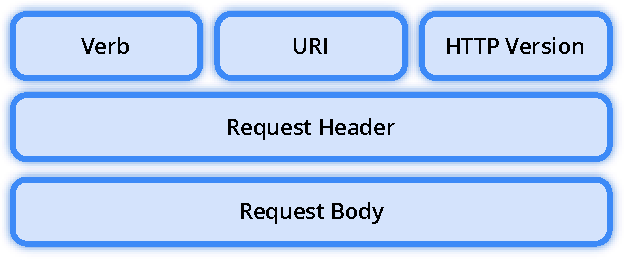
\includegraphics[width=0.5\textwidth]{./figures/http-request.pdf}
	\caption{The~format of~a~HTTP Request.}
	\label{fig-HTTPRequest}
\end{figure}

\begin{enumerate}
  \item Verb indicates the~HTTP method like GET, PUT, POST, etc.
  \item URI is the~Uniform Resource Identifier used to~identify the~resource
  on~the~server.
  \item HTTP version is the~version of~HTTP.
  \item Request header contains metadata as~a~collection of~\uv{key-value} pairs
  of~headers and~their values. For~instance, a~client (or~browser) type, format
  supported by~the~client, format of~the~message body, cache settings
  for~the~response, and~more.
  \item Request body is the~message content or~resource representation.
\end{enumerate}

In~the~listing~\ref{lst-GETRequest} can be seen an~example of~a~request that was
created by~the~browser when it tried to~access the~website of~Faculty
of~Information Technology.

\vspace{1mm}
\begin{lstlisting}[caption=An~example of~a~simplified GET request made
by~the~browser., label=lst-GETRequest, style=dp-default]
GET / HTTP/1.1
Host: www.fit.vutbr.cz
User-Agent: Mozzila/5.0 (Windows NT 6.3; Win64; x64) ...
Accept: text/html,application/xhtml+xml,application/xml; ...
Accept-Encoding: gzip, deflate
Accept-Language: cs-CZ,cs;
\end{lstlisting}

As~can be seen, the~HTTP method is followed by~the~URI and~the~HTTP version.
The~request also contains some headers. For~instance
the~\uv{\textit{User-Agent}} header contains information about the~type
of~a~client which made the~request. The~\textit{Accept} headers tells the~server
about various representation formats, the~encoding, and~a~language the~client
supports. The~server, if it supports more than one representation format, can
decide the~format for~the~response at~runtime depending on~the~value
of~the~\textit{Accept} header.

When the~server receives the~request it responds with~a~HTTP response which
consists of~four major parts as~can be seen
in~the~figure~\ref{fig-HTTPResponse}.

\begin{figure}[!hbt]
	\centering
	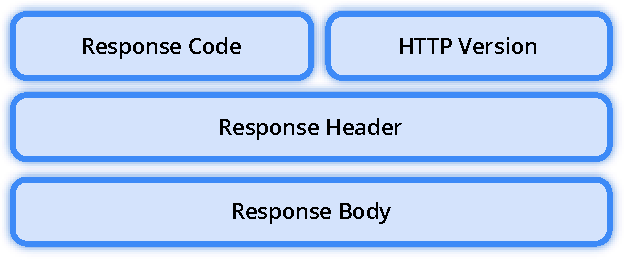
\includegraphics[width=0.5\textwidth]{./figures/http-response.pdf}
	\caption{The~format of~HTTP response.}
	\label{fig-HTTPResponse}
\end{figure}

\begin{enumerate}
  \item Response code contains the~server status for~the~requested resource.
  The~response is a~\uv{3-digit} status code, for~instance, 404 means resource
  not found and~200 means response is ok.
  \item HTTP version is the~version of~HTTP.
  \item Response header contains metadata and~settings of~the~response message
  as~\uv{key-value} pairs. For~example, content type, content language,
  response date, etc.
  \item Response body contains message content or~resource representation if
  the~request was successful.
\end{enumerate}

In~the~listing~\ref{lst-GETResponse} can be seen an~example of~a~response
to~a~request from~the~listing~\ref{lst-GETRequest}. The~response contains
the~version of~HTTP, response code and~several response headers followed
by~the~response body which in~this case is a~HTML page.

\vspace{1mm}
\begin{lstlisting}[caption=An~example of~a~simplified response to~GET
request., label=lst-GETResponse, style=dp-html]
HTTP/1.1 200 OK
Date: Sat, 09 Dec 2017 08:36:01 GMT
Server: Apache
Content-Location: index.php.cz
Pragma: no-cache
Keep-Alive: timeout=60, max=100
Connection: Keep-Alive
Transfer-Encoding: chunked
Content-Type: text/html; charset=iso-8859-2
Content-Language: cs
<!DOCTYPE HTML PUBLIC "-//W3C//DTD HTML 4.01//EN">
<html>
<head>
...
\end{lstlisting}



\subsection{Addressing the Resources}
\label{sec-addressing}
If the~client wants to~get a~resource from~the~server, it needs to~know, how
to~address it. \textit{Addressing} refers to~locating a~resource or~multiple
resources lying on~the~server. It is analogous to~locating a~postal address
of~a~person. A~RESTful service uses directory hierarchy like human readable URIs
to~address its resources. Each resource is identified by~its URI which is
of~the~following format:

\begin{equation}
<protocol>://<serviceName>/<resourceType>/<resourceId>
\end{equation}

However, it needs to~be noted that the~URI should not say anything about
the~operation or~action, because for~identifying the~operation to~be performed
on~the~resource, the~HTTP verbs are used. This enables the~client to~call
the~same URI with different verbs to~perform different operations. The~verbs
correspond to~read, create, update, and~delete\footnote{In~computer
programming, create, read, update, and~delete (as~an~acronym CRUD) are four
basic functions of~persistent storage.} operations. Nevertheless, while
designing URIs there are other practices that should be considered as~well.

\begin{enumerate}
  \item Plural nouns should be used to~define resources.
  \item Spaces should be avoided. Typically in~URIs it's recommended to~use
  underscore or~hyphen when using long resource name.
  \item Lowercase letters are recommended. Although URIs are
  \uv{case-insensitive}, it's a~good practice to~keep them in~lower case letters
  only.
  \item Avoid verbs for~the~resource name until the~resource is actually
  an~operation or~a~process.
\end{enumerate}



\subsection{HTTP Verbs}
\label{lab-verbs}
As~stated in~section~\ref{sec-addressing} the~most used HTTP verbs correspond
to~CRUD operations. For~instance, read operation corresponds to~the~GET verb
which is used to~retrieve a~representation of~a~resource. If the~request is
successful, it returns representation of~the~resource in~a~format that is
accepted by~the~client and~a~response code of~200. Note that the~requests that
utilize the~verb should be used only to~read data, not change it. When used this
way they are considered safe. That is, they can be called without risk of~data
modification or~corruption. Additionally, the~requests are idempotent, which
means that making multiple identical requests ends up having the~same result
as~a~single request.

For~creating resources, the~POST is most often utilized. On~successful creation,
returning a~\textit{Location} header, with a~link to~the~created resource,
and~the~201 response code. The~method is neither safe nor idempotent. Therefore
it is recommended for~\uv{non-idempotent} resource requests. Making two
identical POST requests will most likely result in~two resources containing same
information.

For~update capabilities, the~PUT verb is ofter most utilized, \uv{PUT-ing}
to~a~known resource with the~request body containing the~newly updated
representation of~the~original resource. On~successful update, the~server should
return the~200 or~204 status code if not returning any content in~the~body. It
follows from the~above that a~body in~the~response is optional -- providing one
is not necessary and~only leads to~more bandwidth consumption. The~PUT is not
a~safe operation, in~that it modifies state on~the~server, but is idempotent.
In~other words, if the~resource is updated using the~PUT method and~then
the~same call is made again, the~resource is still there and~has the~same state
as~it did with~the~first call.

The~DELETE verb is pretty straightforward, it is used to~delete a~resource.
On~successful deletion, the~server should return response code of~204 with no
response body. \uv{HTTP-spec-wise}, the~operations are idempotent. If
the~resource is deleted, it is gone. Repeatedly calling the~method on~that
resource ends up the~same -- the~resource is gone. However, there is a~caveat
about the~method's idempotence. Calling it on~the~resource a~second time will
result in~404 response code since the~resource was already removed and~therefore
is no longer findable. It makes the~operation in~fact no longer idempotent,
however, the~\uv{end-state} of~the~resource is the~same.



\subsection{Representation of the Resources}
It is clear that the~focus of~RESTful services is on~resources and~on~providing
access to~them. A~resource can easily be thought of~as~an~object
as~in~OOP\footnote{Object oriented programming (OOP) is a~programming paradigm
based on~the~concept of~\textit{objects}, which may contain data, in~the~form
of~fields; and~code, in~the~form of~procedures, often known as~methods.}.
The~resources can be text files, HTML pages, images or~videos and~can consist
of~other resources. The~server simply provides access to~the~resources
and~client accesses and~modifies them. It is important to~point out that
the~architecture does not put a~restriction on~the~format of~a~resource
representation. However, as~mentioned before, the~most popular representation
formats are XML and~JSON.

\vspace{1mm}
\begin{lstlisting}[caption=An~example of~a~XML representation
of~a~\textit{user} resource., label=lst-XMLExample, style=dp-xml]
<user>
	<id>1</id>
	<firstName>John</firstName>
	<lastName>Doe</lastName>
	<age>42</age>
</user>
\end{lstlisting}

Once a~resource is identified then its representation is to~be decided using
a~standard format so that the~server can send the~resource in~the~above said
format and~the~client can understand said format.

\vspace{1mm}
\begin{lstlisting}[caption=An~example of~a~JSON representation
of~a~\textit{user} resource., label=lst-JSONExample, style=dp-default]
{
	"id": 1,
	"firstName": "John",
	"lastName": "Doe",
	"age": 42
}
\end{lstlisting}

Despite the~fact that there are no restrictions on~the~format of~a~resource
representation, following some important points should be considered.
For~instance, both the~server and~the~client should be able to~understand said
format. Moreover the~format should be able to~represent the~resource completely.



\section{Introduction to~Application Programming Interfaces}
In~computer programming an~application programming interface is the~defined
interface through which interactions happen between an~enterprise and~users
of~its assets. It can become the~primary entry point for~enterprise service,
for~its own website and~applications, as~well as~for~a~partner and~customer
integrations. It is defined through a~contract so~that any application can use
it with relative ease. 

The~API~\cite{RESTfulAPI} approach creates a~loosely coupled architecture that
allows a~component service to~have a~wide range of~future uses, and~is
technology agnostic. The~architecture resolves around providing programmable
interfaces to~a~set of~services to~different applications serving different
kinds of~customers. It assumes that these user groups might change or~evolve
over time in~the~way they utilize the~provided services. The~strategy
of~providing APIs leads to~the~following benefits:

\begin{enumerate}
  \item With~APIs, computers rather than people can manage the~work. Through
  them, companies can update work flows to~make them quicker and~more
  productive.
  \item They allow content to~be embedded from~any site or~application more
  easily. This guerantees more fluid information delivery and~an~integrated user
  experience.
  \item Using APIs, any user or~company can customize the~content and~services
  that they use the~most.
  \item They represent a~cheaper way of~building applications by~increasing
  the~reuse of~services. Providing a~usage or~\uv{analytics-based} evolutionary
  development platform decreases cost of~development and~change to~services.
  \item The~company that releases the~API allows its customers to~access their
  conferencing services in~new, more efficient ways, increasing brand
  recognition and~customer loyalty.
\end{enumerate}



\subsection{When is API RESTful?}
The~previous sections explained the~principles of~RESTful web services
and~introduced the~term Application Programming Interface. However, it is
necessary to~point out that not all web APIs are considered RESTful. An~API is
RESTful only when it is acting under the~REST constraints at~all times. These
constraints restrict the~ways that the~server may process and~respond to~client
requests so~that, by~operating within these constraints, the~service gains
desirable \uv{non-functional} properties, such~as~performance, scalability,
portability and~reliability. These formal constraints are as~follows:

\begin{enumerate}
  \item \textbf{\uv{Client-Server}} -- the~constraint is based
  on~the~separation of~concerns principle. Separating the~user interface
  concerns from the~data storage concerns improves the~portability of~the~user
  interface across multiple platforms.
  \item \textbf{Stateless} -- communication between client and~server have~to be
  stateless. It means that each request from~client to~server must contain all
  the~necessary information to~complete the~transaction. The~main advantage
  of~this approach is that the~system is able to~scale better because the~server
  does not have to~store client state between requests.
  \item \textbf{Cacheable} -- the~constraint ensures that the~clients can cache
  response to~improve performance. \uv{Well-managed} caching partially
  or~completely eliminates some \uv{client-server} interactions, further
  improving scalability and~performance.
  \item \textbf{Uniform Interface} -- in~order to~have efficient caching
  in~a~network, components have~to be able to~communicate via a~uniform
  interface.
  The~definition of~uniform interface consists of~four other constraints,
  however most of~them can be found implemented in~the~HTTP protocol.
  \item \textbf{Layered System} -- in~a~layered system, intermediaries, such
  as~proxies can be placed between client and~server utilising the~web's uniform
  interface. The~main advantage is that intermediaries can then intercept
  \uv{client-server} traffic for~a~specific purposes; for~example caching.
  \item \textbf{Code On Demand} -- it is an~optional constraint and~it allows
  clients to~download programs for~\uv{client-side} execution. The~best examples
  for this are compiled components such~as~Java applets or~\uv{client-side}
  scripts such~as~JavaScript.
\end{enumerate}



\section{The~Importance of~API Testing}
\label{frameworks}
Software testing is an~important phase of~the~software development life cycle
in~general, with~API testing being one of~its most challenging
parts~\cite{TestingAPI}. It is being more~and~more recognised as~being more
suitable for~test automation and~continuous testing than other forms of~testing.
Many~developer teams are starting to~increase the~level of~API testing while
decreasing their reliance on~GUI testing because the~tests at~the~API layer are
less brittle and~easier to~maintain even thought they have to~cover
individual functionalities as~well~as~series or~chain of~functionalities.

In~general the~API testing is used to~determine whether the~APIs
and~the~integrations they enable work in~the~most optimal manner e.g. whether
they return the~correct response, react properly to~edge cases, delivery
responses in~an~acceptable amount of~time, and~respond securely to~potential
security attacks. On~particular, the~testing concentrates on~using software
to~make API calls in~order to~receive an~output before observing and~logging
the~system's response. This enables to~test if the~API returns a~correct
response or~output under varying conditions. The~output is typically a~pass
or~fail status, date, information or~a~call to~another API. However it is
important to~point out that there could be no output at~all or~something
completely unpredicted can occur.

Overall, it's very clear that the~risk of~putting a~bad and~especially insecure
product on~the~market is greater than the~cost to~test it which is why the~API
testing is crucial part of~the~application development process.



\subsection{Beginning with cURL}
As~APIs are becoming an~integral part of~how software works it is not
a~surprise that many frameworks and~applications for~theirs testing were
developed. Probably the~oldest of~them is cURL~\cite{cURL}. It is a~command line
tool for~transferring data using various protocols. It consists of~two products
--~libcurl and~curl. Libcurl is a~\uv{client-side} transfer library with~support
for~a~wide range of~protocols. It is portable, \uv{thread-safe}, feature rich,
and~well supported on~virtually any platform. On~the~other hand, curl is
a~command line tool for~getting or~sending files using URL syntax. Since curl
uses libcurl, it supports the~same range of~common Internet protocols that
libcurl does. In~general, it provides a~generic, language agnostic way
to~demonstrate HTTP requests and~responses.

In~addition, as~REST follows the~same model as~the web, it is possible to~type
an~HTTP address to~the~curl and~use it to~make an~HTTP request to~a~resource
on~a~server. The~server returns a~response, which would typically be converted
by~the~browser to~a~more visual display, as~a~raw code to~show the~developers
what they are really retrieving. Obviously, the~requests that can be made
with~the~tool may test various functionalities such as~sending requests using
various HTTP verbs, specifying query strings and~parameters or~even using
authentication.

\vspace{1mm}
\begin{lstlisting}[caption=An~example of~POST request that creates
\textit{user} resource on~the~server using API endpoint \textit{/users}.,
label=lst-cURL-POST, style=dp-no-strings, language=XML]
curl --request POST \
  --url https://localhost:8080/users \
  --header 'authorization: Bearer {{AcessToken}}' \
  -d '{
  	"firstName": "John", \ 
  	"lastName": "Doe", \
  	"age": 42 \
  }'
\end{lstlisting}

However, it is a~little cumbersome to~work directly with curl, since even
a~simple curl request may look like in~the~listing~\ref{lst-cURL-POST}.
Therefore, other frameworks and~applications, such as~Postman, were developed.



\subsection{Continuous Testing with Postman}
Postman is a~useful tool for~testing the~functionality of~API endpoints. It has
a~nice UI, which makes it easy to~add or~remove parameters, define headers,
authorization methods, and~data without the~hassle of~writing code. It also
allows developers to~create various environments, variables, and~to~save
requests, which curl is not designed to~do.

Besides providing a~friendly user interface for~constructing HTTP requests,
Postman also gives developers the~ability to~write tests against the~responses
of~requests to~see if the~server is returning the~correct results. Requests
constructed in~Postman can also be bundled into a~collection and~easily exported
or~shared, making Postman great for~collaborating on~and~sharing API
specifications with~other developers. In~addition, the~collections can also be
used with~continuous integration systems so that the~same collection used
to~test an~API locally while developing can also be used to~determine whether
or~not the~codebase should be pushed live onto production.

However, there is a~problem with~using Postman for~continuous testing,
because as~was stated in~the~section~\ref{lab-verbs}, not all HTTP verbs are
idempotent. To~clarify, what if a~developer creates a~test that removes
a~resource with~specified identifier from~a~database? If the~code covered
by~the~test is bugfree then the~resource is removed and~the~test successful.
Nevertheless, running the~test repeatedly will result in~the~test's failure
as~the~resource no longer exist. The~solution would be to~create a~test case
that calls the~endpoint which creates the~resource, and~then using the~resource
identifier from~the~response to~remove it. Unfortunately, Postman or~any other
similar application does not allow to~use request's response as~an~input
of~another request.



% =============================================================================



\chapter{Technologies and Frameworks}
\label{Technologies}
In~this chapter are discussed the~details of~technologies and~frameworks that
were used for~the~development of~the~Restty aplication. In~the first sections is
introduced the~Java language and~the~Spring and~Hibernate frameworks that were
used for~building the~backend of~the~application. Following the~thesis
the~frontend web application framework Angular along with~the~superset
of~EcmaScript~6 --~the~TypeScript language is presented, as~well~as~the~web
framework PatternFly and~its key features. Finally, the~last section covers
the~Swagger framework and~its usage within the~Restty application.



\section{Introduction to Java}
The~Java language project was initiated in~June 1991 by~J.~Gosling~\cite{Java}
for~use in~one of~his \uv{set-top} box projects. The~language, initially called
\textit{Oak}, ended up later being renamed as~Java when it was first publicly
released by~Sun Microsystems in~1995. The~language promised \uv{Write Once, Run
Anywhere} (WORA), meaning that compiled Java code can run on~all platforms that
support Java without the~need for~recompilations.

The~WORA is achieved by~compiling the~Java language code to~an~intermediate
representation called Java bytecode, instead of~compiling the~code directly
to~architecture specific machine code. When compiled, the~bytecode is executed
by~a~Java Virtual Machine, which is a~separate program that is optimized
for~the~specific platform on~which the~Java code is run.

\begin{figure}[!hbt]
	\centering
	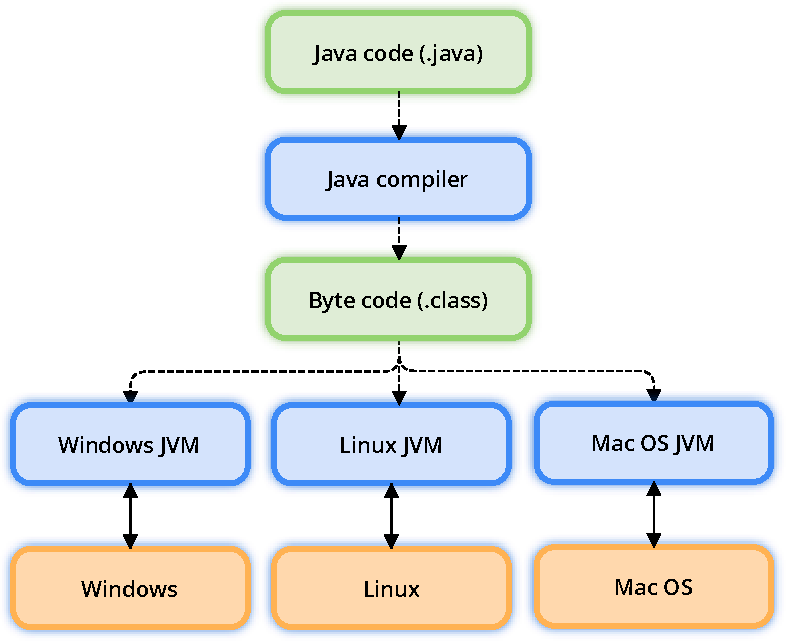
\includegraphics[scale=0.7]{./figures/java-jvm.pdf}
	\caption{Illustration how Java ensures the~\uv{Write Once, Run Anywhere}
	property.}
\end{figure}

However, the~Java's portability is not its only advantage over~other languages
that can be used to~build backend of~a~web application. For~instance, among
the~other benefits belongs the~automatic storage management, strong typing, 
flexible namespace, or~standards for~connectivity to~relational databases.

To~clarify, automatic storage management means that the~JVM automatically
performs all memory allocation and~deallocation while the~program is running.
The~developers cannot explicitly allocate memory for~new objects or~free memory
for~objects that are no longer referenced. Instead, they depend on~a~JVM
to~perform these operations. The~process of~freeing memory is known as~garbage
collection.

In~addition, Java's flexible namespace makes it perfect for~writing complex
applications. That is because Java defines classes and~places them within
a~hierarchical structure that mirrors the~domain namespace of~the~Internet,
which avoids name collisions and~allows Java applications to~be distributed. 



\subsection{Basics of~Java's syntax}
The~syntax of~Java is largely influenced by~C++. However, unlike C++, which
combines the~syntax for~structured, generic, and~\uv{object-oriented}
programming, Java was built almost exclusively as~an~\uv{object-oriented}
language. All code is written inside classes, and~every data item is an~object,
with~the~exception of~the~primitive data types such~as~integers, characters
and~boolean values, which are not objects for~performance reasons.

Following the~above, a~Java program can be defined as~a~collection of~objects
that communicate via invoking each other's methods. To~clarify, object is
an~instance of~a~class, which is a~template that describes the~behavior
and~state that the~object of~its type supports. The~behavior is described via
methods, where the~logics are written, data is manipulated and~all the~actions
are executed.

Nevertheless, as~was mentioned above, Java was influenced by~C++ therefore it is
not a~surprise that the~syntax is similar. However, there are some differences.

\begin{enumerate}
  \item Java is case sensitive, which means identifier \textit{Hello}
  and~\textit{hello} would have different meaning in~Java.
  \item For~all class names, the~first letter should be in~upper case. If
  several words are used to~form a~name of~the~class, each inner word's first
  letter should be in~upper case.
  \item All method names should start with a~lower case letter. If several words
  are used to~form the~name of~the~method, then each inner word's first letter
  should be in~upper case.
  \item Name of~the~class file should exactly match the~class names. That is
  because if~the~file name and~the~class name do not match, the~program will not
  compile.
\end{enumerate}

Overall the~Java's syntax and~best practices are quite extensive, starting
with~basics like identifiers, modifiers, arrays or~interfaces and~ending
with~more advanced features like generics, annotations and~lambda expressions
that were added to~the~language specification over~the~years. Unfortunately,
these specifications are not the~subject of~the~thesis to~be explained
in~detail.



\section{Building a RESTful Web Service}
Even though Java is powerful language, building a~backend of~an~enterprise
application in~plain Java is no easy task. Fortunately, there are many libraries
and~frameworks that provides a~way of~creating high performing, testable web
applications with ease. One of~the~most popular is~the~Spring
Framework~\cite{Spring}, which is an~open source Java platform, initially
released in~June 2003. Spring can be used for~development of~any Java
application, but shines when used for~building web applications on~top
of~the~Java~EE platform. Spring targets to~make J2EE development easier to~use
and~promotes good programming practices by~enabling
a~\uv{POJO-based\footnote{In~software engineering, a~Plain Old Java Object
(POJO) is an~ordinary Java object, not bound by~any special restriction and~not
requiring any class path.}} programming model.



\subsection{The~Advantages of Using Spring Framework}
First and~foremost, the~technology that Spring is most identified with~is
the~Dependency Injection (DI) flavor of~Inversion of~Control (IoC). The~IoC is
a~general concept, and~it can be expressed in~many different ways. Dependency
Injection is merely one concrete example of~IoC.

When writing complicated Java application, the~application classes should be
as~independent as~possible of~other Java classes to~increase the~possibility
to~reuse these classes and~to~test them independently of~other classes while
unit testing. Dependency Injection helps in~gluing these classes together
and~at~the~same time keeping them independent. To~clarify, consider
an~application which has a~text editor component and~the~developer wants
to~provide a~spell check to~said component. The~standard code would look similar
to~the~code in~the~listing~\ref{lst-spring-di-1}, creating a~dependency between
\textit{TextEditor} and~the~\textit{SpellChecker} classes.

\vspace{1mm}
\begin{lstlisting}[caption=The~standard way of~providing spell checking
to~a~component., style=dp-default, language=Java, label=lst-spring-di-1] 
public class TextEditor {

	private SpellChecker spellChecker;
	
	public TextEditor() {
		this.spellChecker = new SpellChecker();
	}
	
}
\end{lstlisting}

As~can be seen in~the~listing~\ref{lst-spring-di-2}, in~an~inversion of~control
scenario, the~developer would create code differently, in~this scenario
the~total control was removed from~the~\textit{TextEditor} class
and~the~dependency (i.e. \textit{SpellChecker} class) is being injected into
the~\textit{TextEditor} through a~class constructor. Thus the~flow of~control
has been \uv{inverted} by~Dependency Injection because the~developer effectively
delegated dependencies to~an~external system.

\pagebreak
\begin{lstlisting}[caption=The~Inversion of~Control scenario of~providing
a~\textit{SpellChecker} to~the~\textit{TextEditor} component., style=dp-default,
language=Java, label=lst-spring-di-2]
public class TextEditor {

	private SpellChecker spellChecker;
	
	public TextEditor(SpellChecker spellChecker) {
		this.spellChecker = spellChecker;
	}
	
}
\end{lstlisting}

The~other key~advantage of~Spring is the~Aspect Oriented Programming (AOP)
framework. AOP entails breaking down program logic into distinct parts called
concerns. The~functions that span multiple points of~an~application are called
\uv{cross-cutting} concerns and~are conceptually separate from~the~application's
business logic. As~mentioned earlier, the~key unit of~modularity in~OOP is
the~class, whereas in~AOP the~unit of~modularity is the~aspect, which is
the~combination of~the~pointcut and~the~advice~\footnote{Advice describes
a~class of~functions which modify other functions when the~latter are run.}.
As~DI helps decouple the~application objects from~each other, AOP helps decouple
\uv{cross-cutting} concerns from~the~objects that they affect. To~clarify,
the~AOP module provides interceptors to~intercept an~application meaning when
a~method is executed, the~developers have the~option to~add an~extra
functionality before or~after the~method execution using the~interceptors.



\section{Persisting Data With Hibernate}
Even though the~Spring Framework covers a~lot of~functionality needed to~build
complex web application and~adds significant enhancements to~the~data access
layer of~Java language, it is still best to~use external
ORM\footnote{\uv{Object-relational} mapping (ORM) is a~programming technique
for~converting data between incompatible type systems using
\uv{object-oriented} programming languages.} framework. For~the~development
of~the~Restty application I've chosen to~use the~Hibernate
framework~\cite{Hibernate} on~top of~the~PostgreSQL database.

Hibernate is a~high performance ORM solution for~Java, created by~G.~King
in~2001. Hibernate maps Java classes to~database tables ~Java data types to~SQL
data types and~relieves the~developer from~most of~common data persistence
related programming tasks. Hibernate consists of~layered architecture which
helps the~developer to~operate without having to~know the~underlying APIs. It
makes use of~the~database and~configuration data to~provide persistence services
(and~persistent objects) to~the~application. The~entire concept of~Hibernate is
to~take the~values from~Java class attributes and~persist them to~a~database
table. To~provide such functionality, the~classes should follow specific rules.

\begin{enumerate}
  \item A~class that will be persisted needs a~default constructor.
  \item All classes should contain an~ID in~order to~allow easy identification
  of~the~objects within Hibernate and~the~database. The~ID property is mapped
  to~the~primary key of~a~database table.
  \item All attributes that will be persisted should be declared private
  and~have appropriate getters and~setters defined in~the~JavaBean style.
\end{enumerate}

\begin{figure}[!hbt]
	\centering
	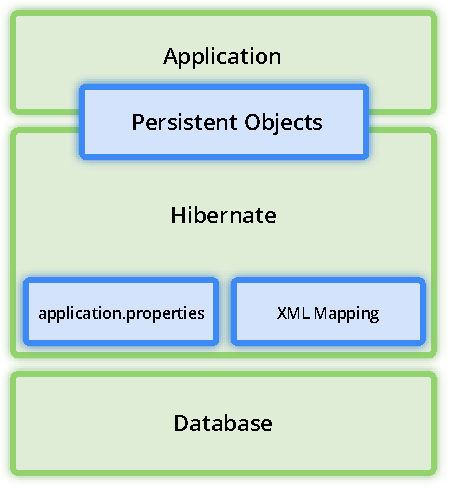
\includegraphics[scale=0.8]{./figures/hibernate-architecture.pdf}
	\caption{High level view of~the~Hibernate framework architecture.}
\end{figure}

As~can be seen in~the~listing~\ref{lst-table}, a~class is mapped to~the~database
using Hibernate annotations on~the~entity. Hibernate's annotations are a~way
of~providing the~metadata for~the~ORM mapping. All the~metadata is clubbed
into~the~POJO Java file along with~the~code, which helps the~developer
to~understand the~table structure and~POJO simultaneously during
the~development.

\vspace{1mm}
\begin{lstlisting}[caption=POJO class that features the~advantages of~ORM.,
style=dp-default, language=Java, label=lst-table]
@Entity
@Table("users")
@SequenceGenerator(name = "users_id_sequence", allocationSize = 1)
public class User {

	private Long id;
	private String name;
	
	@Id
	@Column(name = "id")
	@GeneratedValue(strategy = SEQUENCE, generator = "users_id_sequence")
	public Long getId() {
		return id;
	}
	
	public void setId(Long id) {
		this.id = id;
	}
	
	@Column(name = "name")
	public String getName() {
		return name;
	}
	
	public void setName(String name) {
		this.name = name;
	}

}
\end{lstlisting}

When mapping the~entity, Hibernate detects the~annotations and~accesses
the~properties through getter and~setter methods by~default. The~primary key
of~the~table is determined by~the~\textit{@Id} annotation, which by~default will
automatically determine the~most appropriate primary key generation strategy
to~be used. However, the~default generation strategy can be overriden
by~applying the~\textit{@GeneratedValue} annotation, which takes two
parameters~--~strategy and~generator.

\vspace{1mm}
\begin{lstlisting}[caption=The~SQL code that is generated by~Hibernate when
mapping the~entity from~the~listing~\ref{lst-table}, style=dp-default,
language=SQL, label=lst-table-sql]
CREATE TABLE public.users
(
	id bigint NOT NULL,
	name character varying(255,
	CONTRAINT users_pky PRIMARY KEY (id)
)
\end{lstlisting}

The~second advantage of~using Hibernate is Hibernate Query Language (HQL) which
is an~\uv{object-oriented} query language, similar to~SQL, but instead
of~operating on~tables and~columns, HQL works with~persistent objects and~their
properties. The~queries are translated by~Hibernate into~conventional SQL
queries, which in~turns perform an~action on~the~database. Although it is
possible to~use SQL statements directly with~Hibernate's Native SQL, it is not
recomennded because of~possible database portability hassles and~Hibernate's SQL
generation and~caching strategies.

\vspace{1mm}
\begin{lstlisting}[caption=An~example of~HQL query that selects users with~name
\uv{John Doe}., style=dp-default, language=Java, label=lst-hql] 
StringBuilder hql = new StringBuilder(" FROM ");
hql.append(User.class.getName());
hql.append(" WHERE name = :name ");

Query query = session.createQuery(hql.toString());
query.setString("name", name);
return query.list();
\end{lstlisting}



\section{What is Angular?}
Angular~\cite{Angular} is an~open source TypeScript framework used to~build web
applications in~HTML and~TypeScript. It makes it easy to~build an~application
as~it combines declarative templates, dependency injection, \uv{end-to-end}
tooling, and~integrated best practices to~solve development challenges.


\subsection{Beginning as AngularJS}
Angular originally started as~AngularJS, it was developed in~2009
by~M.~Hevery~\cite{HeveryAngularJS} as~the~software behind an~online JSON
storage service that would have been priced by~the~megabyte,
for~\uv{easy-to-make} applications for~the~enterprise. However, the~business
idea was soon abandoned and~AngularJS was released as~an~open source library
in~October 2010.

The~framework was used to~overcome obstacles encountered while working
with~Single Page applications\footnote{A~single page application (SPA) is a~web
application or~web site that interacts with the~user by~dynamically rewriting
the~current page rather than loading entire new pages from a~server.}.
However, because some of~the~core assumptions in~AngularJS needed to~be changed,
in~September 2016 saw the~light of~the~day a~complete rewrite of~AngularJS.
Originally, the~rewrite was called \uv{Angular 2} by~the~team that built it, but
this led to~confusion among developers. To~clarify, the~team announced that
separate terms should be used for~each framework with \uv{AngularJS} referring
to~the~1.X versions and~\uv{Angular} without the~\uv{JS} referring to~version~2
and~up.

As~the~new version of~the~framework was developed, some new concepts appeared.
In~addition to~better \uv{event-handling} capabilities, powerful templates,
and~better support for~mobile devices, Angular introduced several new features.

\begin{enumerate}
  \item The~earlier version of~Angular had a~focus of~controllers, but now has
  changed the~focus to~having components over controllers. Components help
  to~build applications into many modules which helps in~better maintaining
  the~application over~a~period of~time.
  \item The~newer version of~Angular is based on~TypeScript which is a~superset
  of~JavaScript, maintained by~Microsoft. More information about TypeScript will
  be provided later in~the~section~\ref{TypeScript}.
  \item The~newer version of~Angular introduced services which are a~set of~code
  that can be shared by~different components of~an~application. For~instance,
  consider a~data component that picks data from~a~database, it is possible
  to~have it as~a~shared service that could be used across multiple
  components.
\end{enumerate}


\subsection{Angular's Core Concepts}
As~mentioned in~previous section, Angular introduces the~two core concepts
--~components and~services, respectively the~dependency injection. An~Angular
application will always have a~root component that contains all other
components. In~other words, an~application will always have a~component tree,
in~which components are~a~logical piece of~code that consists of~following
parts:

\begin{enumerate}
  \item Templates that are used to~render the~view for~the~application. They
  contains the~HTML that needs to~be~rendered as~well as~the~bindings
  and~directives.
  \item Classes that are like a~classes defined in~any language, such~as~C,
  except they are defined in~TypeScript. Classes contains properties, methods,
  and~the~code which is used to~support the~view.
  \item Metadata that contains an~extra data defined for~the~Angular class. They
  are defined using a~decorator.
\end{enumerate}

To~clarify, consider an~example from~the~listing~\ref{lst-angular-component}
which contains all three parts. It defines a~class called
\textit{HelloWorldComponent} which contains only one property --~\textit{title}.
The~component is then defined using the~\textit{@Component} decorator that
contains HTML template which is the~view that needs to~be rendered
in~the~application.

\pagebreak
\begin{lstlisting}[caption=An~Angular class with~the~\textit{@Component}
decorator and~a~HTML template., label=lst-angular-component, style=dp-default,
language=Java]
@Component ({
	selector: 'my-app-hello-world',
	template: `
		<div>
			<h1>{{title}}</h>
		</div>
	`,
})
export class HelloWorldComponent {
	title: string = 'Hello World!';
}
\end{lstlisting}

The~second cornerstone of~an~Angular application is dependency injection.
The~idea behind it is pretty simple. If a~component that depends on~a~service is
needed, the~developers do not create the~service by~themselves. Instead they
request one in~the~constructor and~the~framework will provide one. This approach
leads to~more decoupled code which enables testability and~easier maintainence.

\begin{figure}[!hbt]
	\centering
	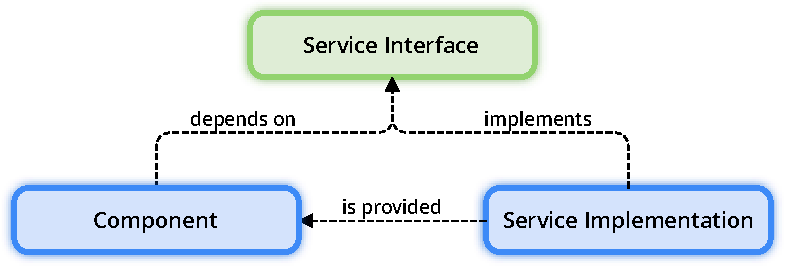
\includegraphics[scale=0.8]{./figures/dependency-injection.pdf}
	\caption{Angular's way of~injecting and~instantiating services
	in~the~components.}
	\label{fig-dependency-injection}
\end{figure}

To~clarify, consider an~example from~the~listing~\ref{lst-angular-service}.
The~listing contains a~simplified service that has a~method that returns
an~array of~users. If a~component is created and~an~argument
of~type~\textit{UserService} is passed to~the~component's constructor
as~a~parameter, Angular automatically instantiates and~injects the~service
into~the~component. 

As~can be seen, the~Angular's dependency injection module is flexible, and~easy
to~use because the~objects can be injected only via constructors. In~addition,
the~injectors form a~hierarchy, and~the~injectable object does not have to~be
an~\uv{application-level} singleton as~it might by~default in~Spring
framework\footnote{Spring framework is an~application framework and~inversion
of~control container for~the~Java platform that relies heavily on~dependency
injection.}.
\pagebreak

\begin{lstlisting}[caption=An~example of~dependency injection in~Angular.,
label=lst-angular-service, style=dp-default, language=Java]
export class UserService {
	users: User[] = [];
	
	findUsers(): User[] {
		// Code used to retrieve the users
		return users;
	}
}


@Component {
	...
}
export class UsersComponent {
	users: User[] = [];
	
	constructor(userService: UserService) {
		this.users = userService.findUsers();
	}
}
\end{lstlisting}


\section{Introducing~TypeScript}
\label{TypeScript}
In~september 1995 was first introduced JavaScript as~a~language for~the~client
side. It was used to~make webpages interactive and~to~provide online programs,
including video games. However, as~JavaScript code grows, it tends to~get
messier, making it difficult to~maintain and~reuse. Moreover, its failure
to~embrace the~features of~Object Orientation, strong type checking
and~\uv{compile-error} checks prevent JavaScript from~succeeding
at~the~enterprise level as~a~\uv{full-fledged} server side technology.
TypeScript was presented to~bridge this gap. Its main goals were to~provide
an~optional type system and~planned features from~future JavaScript editions
to~current JavaScript engines.


\subsection{Why Add Types to JavaScript}
Types have proven ability to~enhance code quality and~understandability.
Increasing the~agility when doing refactoring and~being one of~the~best forms
of~documentation a~developer can have. However, types have a~way of~being
unnecessarily ceremonious. Therefore TypeScript is very particular about keeping
the~barrier to~entry as~low as~possible, only providing compile type safter
for~the~JavaScript code. The~great thing is that the~types are completely
optional.

TypeScript provides data types as~a~part of~its optional type system. As~a~super
type of~all types, the~\textit{any} data type is used. It denotes a~dynamic type
and~using it is equivalent to~opting out of~type checking for~a~variable. That
suggests that the~variable may be declared with no type which means that
the~type of~the~varible will be inferred by~the~TypeScript Language Service.
All~other \uv{built-in} types and~\uv{user-defined} types inherit
from~the~\textit{any} type.

Important to~mention is that the~\uv{built-in} types \textit{undefined}
and~\textit{null} may look similar but are not the~same. A~variable initialized
with~\textit{undefined} means that the~variable has no value or~object assigned
to~it, while \textit{null} means that the~variable has been set to~an~object
whose value is undefined.

\begin{figure}[!hbt]
	\centering
	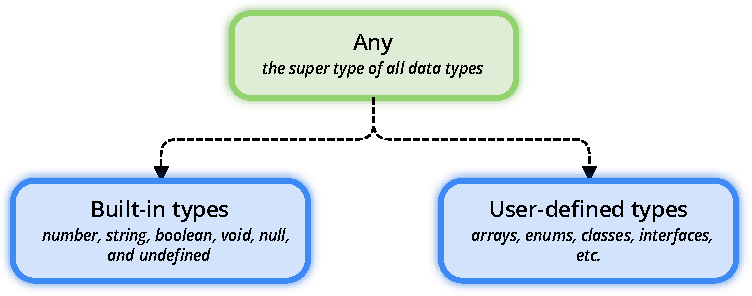
\includegraphics[scale=0.8]{./figures/data-types.pdf}
	\caption{Classification of~data types in~TypeScript.}
	\label{fig-datatypes}
\end{figure}

The~main advantage is however that the~JavaScript code files with the~\uv{.js}
suffix can be renamed to~a~files with \uv{.ts} suffix and~TypeScript will give
back a~valid equivalent to~the~original JavaScript file. That is because
TypeScript is intentionally and~strictly a~superset of~JavaScript with~optional
type checking.


\subsection{Future JavaScript}
The~second goal of~TypeScript was to~provide planned features from~future
JavaScript editions. Nowadays, it provides a~number of~features that are planned
in~EcmaScript~6\footnote{The~EcmaScript specification is a~standardized
specification of~a~scripting language.} for~current JavaScript engines.
For~instance, the~language features modules and~\uv{class-based} orientation
as~well as~features like generics and~type annotations that are not part
of~the~specification.

In~conclusion, even thought we could use JavaScript with Angular, TypeScript
feels like a~superior choice, not only because it is strongly typed and~supports
object oriented programming, but because of~the~TypeScript's transpiler which
provides the~\uv{error-checking} feature. Unlike JavaScript,
the~TypeScript is not an~interpreted language and~will compile the~code
and~generate compile errors if it finds some sort of~syntax errors. Thus
helps to~highlight the~errors before the~script is run hence, saving time trying
to~find the~bugs in~the~code.


\section{Styling with PatternFly}
The~success of~an~application depends on~a~\uv{well-designed} user interface.
The~good or~bad design can influence the~perceived usability of~an~application,
and~if the~application's design is not done well, whole application can be
perceived as~bad. The~PatternFly framework was developed specifically to~address
the~issue.

One of~the~main things that sets the~framework apart from~other libraries, such
as~Bootstrap, is the~focus on~design for~IT enterprise applications. It
recognizes the~importance for~a~user to~be able to~migrate seamlessly from~one
product to~another without having to~relearn the~UI. Behavioral consistency
leads to~better usability because users are familiar with~the~interactions.
Visual consistency establishes a~look and~feel that users recognize and~allows
to~unify disparate projects, make them look great and~make them look like they
belong in~the~same portfolio.

PatternFly is an~open source project that is based
on~Bootstrap~\cite{Bootstrap}, a~\uv{mobile-first} frontend framework
for~creating web sites and~applications. It is developed using Less, a~cascading
style sheet \uv{pre-processor} that extends the~CSS language and~adds features
that allow variables, mixins, functions, and~other techniques that allow
developers create code that is maintainable, themeable and extendible. This
allows the~developers to~add any required \uv{app-specific} CSS directly into
one CSS file, which is more performant, and~make any necessary adjustments
to~PatternFly via variable overrides.

The~framework consists of~a~series of~Less stylesheets that implements various
components of~the~toolkit. The~stylesheets are generally compiled into a~bundle
and~included in~the~applications, however individual components can be included
or~removed. Moreover, the~framework provides a~number of~variables that control
styling of~various components. Each component consists of~a~HTML structure
and~CSS declarations, and~in~some cases accompanying JavaScript code.


\subsection{Using the Components}
The~framework comes by~default with various design templates for~typography,
tables, forms, buttons, and~other interface components that can be used building
the~application --~saving lots of~time and~efforts in~the~development process.
The~templates are made available as~\uv{well-factored} CSS classes that
the~developers can apply to~the~HTML to~achieve different effects. By~using
semantic class name like \textit{.alert} or~\textit{.alert-success},
the~components are easily reusable and~extensible. Although PatterFly uses
descriptive class names that have a~meaning, it is not specific
about~implementation details. Therefore all classes can be overriden with~custom
style and~still, the~meaning of~the~class will remain the~same.

\begin{lstlisting}[caption=An~example of~styling the~component using predefined
class \textit{.alert}., label=lst-alert, style=dp-html]
<div class="container">
	<div class="alert alert-success">
		<span class="pficon pficon-ok"></span>
		<strong>Hello World!</strong>
		<span>This is an example of an alert in PatternFly.</span>
	</div>
</div>
\end{lstlisting}

As~can be seen in~the~figure~\ref{fig-alert}, the~code snippet
from~the~listing~\ref{lst-alert} generates a~component that contains
the~\uv{Hello World!} text. Using the~semantic class names, the~code is easily
styled, allowing the~developer to~spend more time on~application specific
features and~functions rather than application designs.

\begin{figure}[!hbt]
	\centering
	
\includegraphics[scale=0.8]{./figures/patternfly-alert.pdf}
	\caption{Illustration of~a~component styled using the~semantic classes
	from~PatternFly.}
	\label{fig-alert}
\end{figure}

\subsection{Working with the Grid}
In~the~beginning of~this section was mentioned that the~PatternFly, respectively
its predecessor Bootstrap, was developed with~a~\uv{mobile-first} design
philosophy, which resulted in~a~framework that is responsive by~design. The~end
result is that it easily and~efficiently scales with~a~single code base,
from~phones, through tablets, to~desktops. The~responsiveness is achieved using
a~fluid grid system that can be applied to~appropriately scale~up to~12 columns
according to~the~size of~the~device or~viewport. The~grids provides structure
to~the~layout, defining the~horizontal and~vertical guidelines for~arranging
content and~enforcing margins.

To~use the~grid system, a~few rules have to~be followed. Grid column elements
have to~be placed inside row elements, which creates horizontal groups
of~columns. It is possible to~have as~many rows as~needed, but it is necessary
that the~columns are immediate children of~rows. In~a~full row, the~column
widths are any combination that adds up~to~12, however it is not mandatory
to~use all~available columns.

\begin{lstlisting}[caption=An~illustration of~the~grid system in~PatternFly.,
label=lst-grid, style=dp-html]
<div class="container">
	<div class="row">
		<div class="col-md-6">First column</div>
		<div class="col-md-6">Second column</div>
	</div>
	<div class="row">
		<div class="col-md-3">First column</div>
		<div class="col-md-3">Second column</div>
		<div class="col-md-3">Third column</div>
		<div class="col-md-3">Fourth column</div>
	</div>
</div>
\end{lstlisting}

The~rows have to~be places in~a~\uv{fixed-width} layout wrapper that has
a~\textit{.container} class attached and~a~width of~1170px or~in~\uv{full-width}
layout wrapper, which has~\textit{.container-fluid} class attached, and~which
enables the~responsive behavior in~that row. The~grid system is based on~four
tiers of~classes -- \textit{xs} for~phones, \textit{sm} for~tables, \textit{md}
for~desktops, and~\textit{lg} for~larger desktops. These classes define
the~sizes at~which the~columns collapse or~spread horizontally. 


\section{Introduction to Swagger Framework}
Swagger~\cite{Swagger} is an~open source framework for~designing and~describing
APIs. It was developed by~Reverb Technologies in~2010 to~solve the~need
for~keeping the~API design and~documentation in~sync. It provides a~large
ecosystem of~tools that helps developers design, build, document, consume,
and~test RESTful web services. It defines a~standard, language agnostic
interface to~APIs which allows both humans and~machines to~discover
and~understand the~capabilities of~the~service. The~standard is called
the~OpenAPI Specification which is a~specification for~\uv{machine-readable}
interface files. The~files are essentially a~resource listings of~the~API which
adheres to~the~specification. The~files are either of~YAML or~JSON format
and~contains a~detailed description of~the~entire API. Nowadays there are two
ways to~create such file.

\begin{enumerate}
  \item \uv{Top-down} approach, or~\uv{design-first} which means using Swagger
  to~design the~API before writing any actual code.
  \item \uv{Bottom-up} approach, or~\uv{code-first} which means using Swagger
  to~document the~API of~an~existing code.
\end{enumerate}


\subsection{Using the~Swagger}
In~the~past, it was popular to~use the~\uv{code-first} approach which is much
easier because the~developers can make adjustmens on~the~fly, and~it fits nicely
into an~Agile delivery process. But because very often, the~developers are not
thinking about the~design, it can make the~API difficult to~understand
and~document. To~solve this, Swagger supports various annotations, as~can be
seen in~the~listing~\ref{lst-swagger-api}, that allow developers to~specify
the~details of~the~documentation. The~alternative way is to~let Swagger figure
out the~documentation by~itself based on~the~annotations from~Spring
framework\footnote{Swagger is~a~specification, and~supports a~wide range
of~frameworks and~their annotations.}. Under the~hood, it scans Spring
controllers on~\uv{start-up} and~registers a~documentation controller that
exposes the~operations Spring controllers implement. The~documentation follows
the~specification --~any client that understands the~specification can use
the~API. The~important thing is that the~documentation is based on~the~code
itself, therefore any change to~the~code is reflected on~the~documentation.
There is no need to~maintain an~external document.

\vspace{1mm}
\begin{lstlisting}[caption=An~example of~Spring controller with Swagger's
annotations that can be used to~generate API documentation., style=dp-default,
language=Java, label=lst-swagger-api]
@RestController
@RequestMapping("/users")
@Api(value = "users", description = "Users endpoints")
public class UserController {

	@Autowired
	private UserService userService;
	
	@GetMapping
	@ResponseStatus(HttpStatus.OK)
	public List<User> findAll() {
		return userService.findAll();
	}
	
	@PostMapping
	@ResponseStatus(HttpStatus.CREATED)
	public User create(@RequestBody UserDto userDto) {
		return userService.create(userDto);
	}
	
	@DeleteMapping
	@ResponseStatus(HttpStatus.NO_CONTENT)
	@RequestMapping(value = "/users/{userId}")
	public void remove(@PathVariable Long userId) {
		userService.removeById(userId);
	}

}
\end{lstlisting}

On~the~other hand, the~push for~clear, easy to~read documentation has
popularized the~\uv{design-first} approach. Not only more developers can have
input on~the~documentation, but it actually results in~cleaner code, because
the~developers are forced to~think simpler, more concise, and~easy to~follow.
The~framework contains an~editor that allows to~write up~the~documentation
in~appropriate formats and~have it automatically compared against the~Swagger
specification. Any mistakes are flagged, and~alternatives are suggested. This
way, when developers publish the~documentation they can be sure that it's
\uv{error-free}. As~can be seen in~the~listing~\ref{lst-swagger-json},
the~documentation consists of~2 parts, the~operations and~the~models.

In~either case the~framework exposes the~endpoints from~the~documentation
controller and~makes them accessible which allow for~applications to be built
upon the~documentation. The~application that will be developed in~the~thesis
will take an~advantage of~the~exposure. It will take an~existing JSON document
created by~the~framework and~build an~interactive documentation and~testing
environment upon it.

\vspace{1mm}
\begin{lstlisting}[caption=An~example of~API documentation in~JSON format
created using the~Swagger framework., style=dp-default, label=lst-swagger-json]
{
	"apiVersion": "1.0",
	"swaggerVersion": "1.0",
	"basePath": "http://localhost:8080",
	"resourcePath": "/users",
	"apis": [
		{
			"path": "/users",
			"description": "Users endpoints",
			"operations": [
				{
					"httpMethod": "GET",
					"summary": "findAll",
					"deprecated": "false",
					"responseClass": "List[User]", 
				},
				
				... 
			]
		}
	],
	"models": [
		"User": {
			"properties": {
				"id": {
					"type": "long"
				},
				"firstname": {
					"type": "string"
				},
				"lastname": {
					"type": "string"
				}
			}
		}
		
		...	
	]
}
\end{lstlisting}
  


% ==============================================================================



\chapter{Application Design}
\label{Design}
This chapter covers the~requirements for~the~Restty application and~presents
the~application design drafts in~detail. The~design drafts can help reveal any
clashing visual elements while it is still easy to~change them before writing
the~code. Moreove, the~drafts allow to~fully flesh out the~ideas and~choose
the~best possible options. The~design drafts pictured in~the~following sections
consists of~separate UI elements that once combined, represent the~final design
draft of~the~Restty application.


\section{Requirements for~the~Restty Application}
As~mentioned earlier, the~aim of~the~thesis is to~create an~application that
allows to~test single endpoints of~the~interfaces of~other applications
as~well~as to~create extensive test cases from~said interfaces. The~interface
that should be tested will be provided via the~Swagger's JSON file which
contains all necessary information about~the~interface. Therefore the~Restty has
to~allow the~users to~choose the~application's interface upon which will
the~Restty work. If the~interface and~its endpoints is successfully loaded
and~the~data are persisted in~the~Restty's database, the~user should be
redirected to~the~dashboard which should display basic statistics about
the~status of~the~endpoints and~test cases.

From~the~dashboard the~users should be able to~navigate to~the~overview of~all
interface's endpoints, their details, configurations and~past test runs.
In~addition, the~users should be able to~navigate to~the~similar overview
with~test cases, which the~users can create using the~Restty's Test Case
Creator (TCS). The~TCS should allow create test cases that can combine various
endpoints and~other test cases. To~clarify, it should be possible to~test
an~API's endpoint and~use its output as~an~input of~another endpoint.


\section{Designing the~Project Explorer}
The~entry point of~the~application should be the~Project Explorer. The~Project
Explorer should allow users to~create and~manage the~projects created within
the~Restty. Each project should have a~unique name which distinguishes it
in~the~application. When the~project is created by~the~user, besides its name,
it needs to~have specified a~source of~the~project's endpoints. As~a~source
(in~form of~a~URL) is considered Swagger JSON with~information about
the~project's interface. The~source should be then passed to~the~Restty's
backend that should make an~request for~the~interface, parse the~request's
response and~persist the~information about interface's endpoints and~models
to~the~database. If~the~project information are successfully persisted
in~the~Restty's database, the~user should see the~newly added project and~its
attributes, such as~amount of~endpoints and~test cases, in~the~Project
Explorer's list table.

\begin{figure}[!hbt]
	\centering
	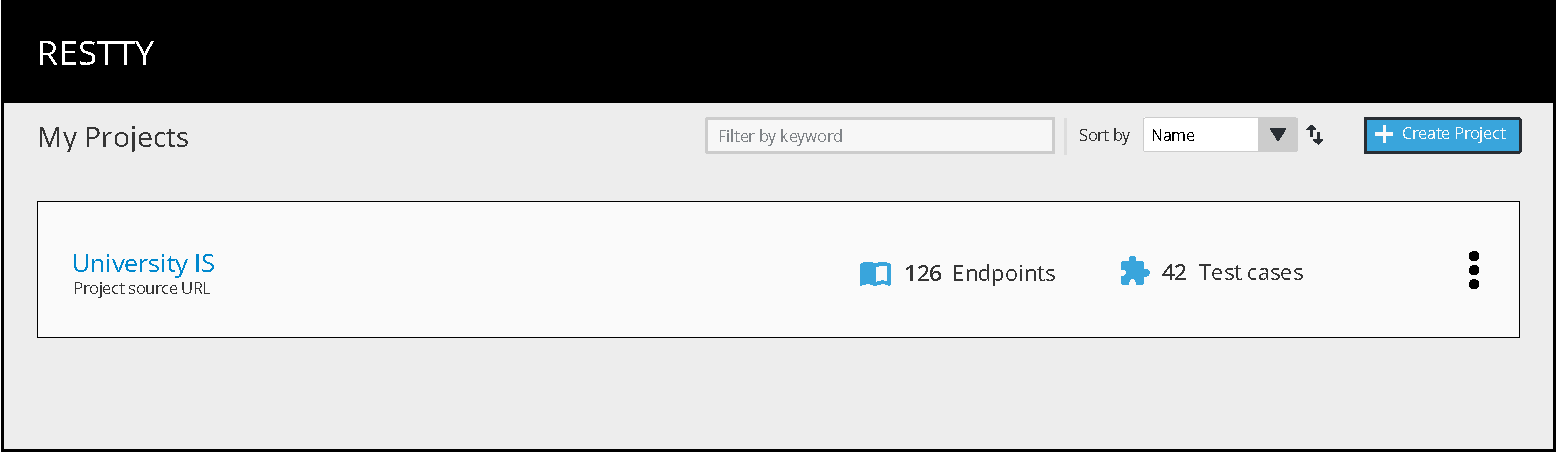
\includegraphics[scale=0.55]{./designs/project-explorer.pdf}
	\caption{The~Project Explorer that contains list of~projects created
	in~the~Restty application.}
\end{figure}

Overall, the~list table should show the~users some basic information about their
projects and~should allow them to~manage them. Finally, by~clicking on~the~list
item the~users should be redirected to~the~specified project's dashboard.


\section{The~Project Dashboard}
The~dashboard is the~entry point of~each specific project. It consists
of~a~horizontal and~vertical navigation bars, donut charts and~tables that
contains latest information about the~project. To~keep things simple,
the~horizontal navigation bar should allow users to~swiftly switch between
projects without the~need to~access the~Project Explorer. On~the~other hand
the~vertical navigation bar should allow users to~quickly navigate between
the~project's endpoints, test cases and~settings.

\begin{figure}[!hbt]
	\centering
	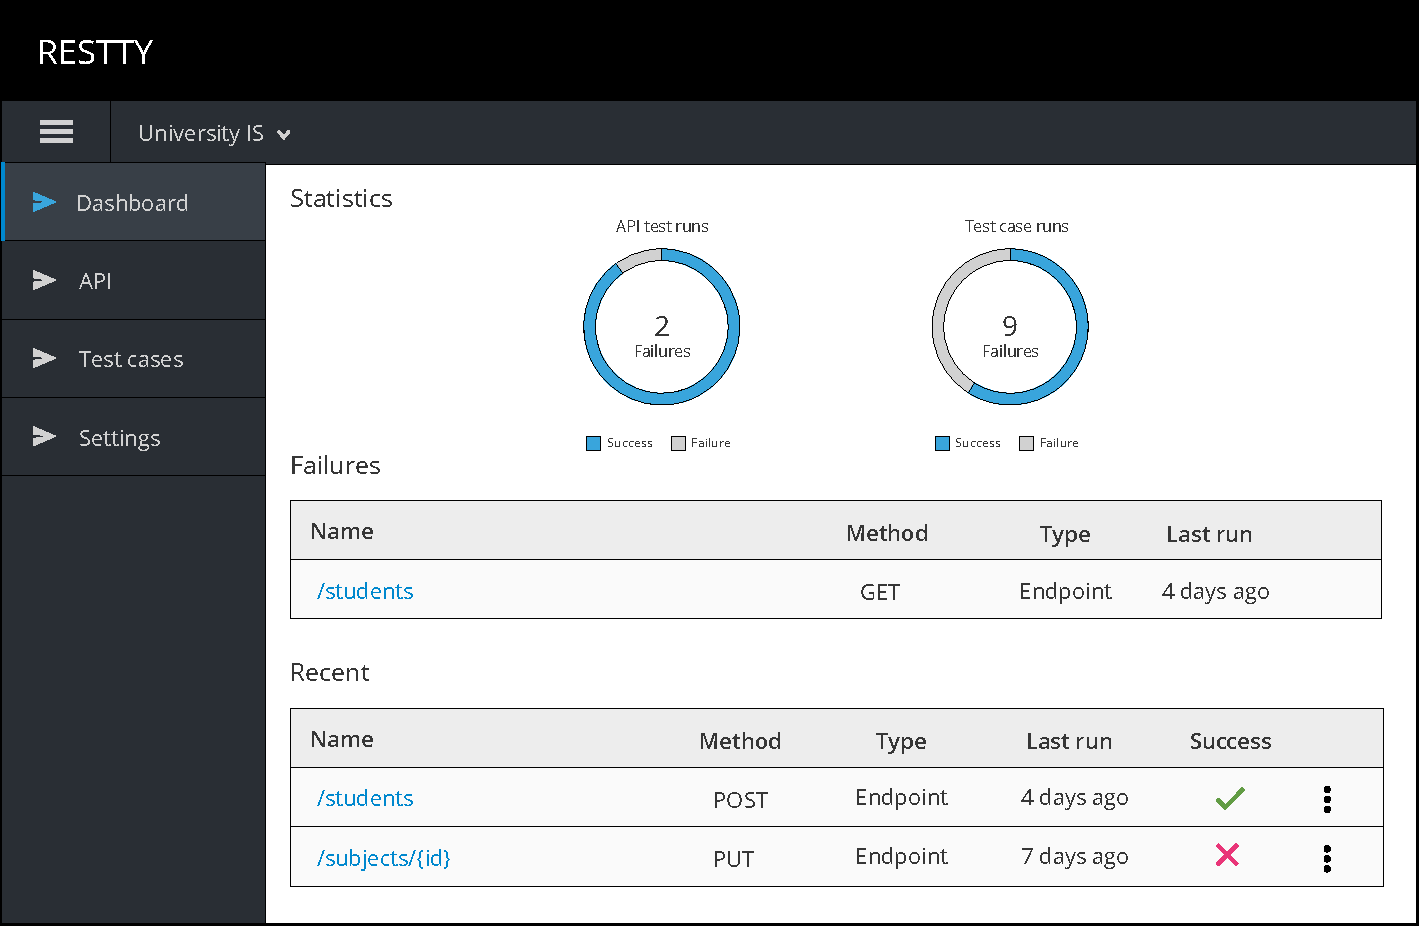
\includegraphics[scale=0.6]{./designs/dashboard.pdf}
	\caption{The~dashboard of~a~project with~lastest information about test runs.}
\end{figure}

Informace o donut charts
Informace o tabulkach

\section{Showing the~Endpoints}
Once the~users choose a~project to~work with~within the~application, they should
be able to~view and~test the~endpoints that are provided by~that project.
However, as~explained in~the~section~\ref{frameworks}, many applications which
provide an~overview of~an~API's endpoints does not scale well enough if they
encounter large amount of~the~endpoints. To~address this issue, in~the~thesis
was used for~the~presentation of~the~APIs a~\uv{tree-like} structure.

\begin{figure}[!hbt]
	\centering
	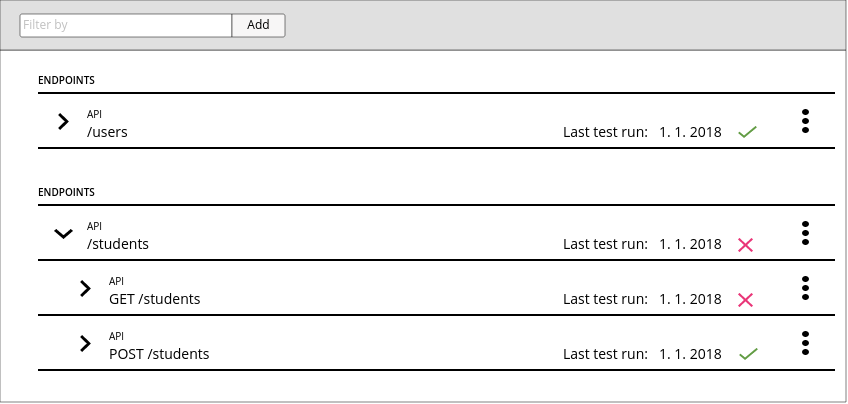
\includegraphics[scale=0.4]{./designs/drafts-1.0/api-general.png}
	\caption{The~overview of~an~API's endpoints ordered into~a~hierarchical
	\uv{tree-like} structure.}
	\label{api-general}
\end{figure}

As~~can be seen in~figure~\ref{api-general} by~default only \uv{top-level} nodes
of~the~tree are shown. However, the~users can then expand the~nodes and~view
details of~particular endpoints or~run tests using the~settings menu in~the~top
right corner of~the~endpoint node. Once the~user encounters the~leaf node,
the~information about that particural leaf node are shown in~detail as~can be
seen in~the~figure~\ref{api-detail}.

\begin{figure}[!hbt]
	\centering
	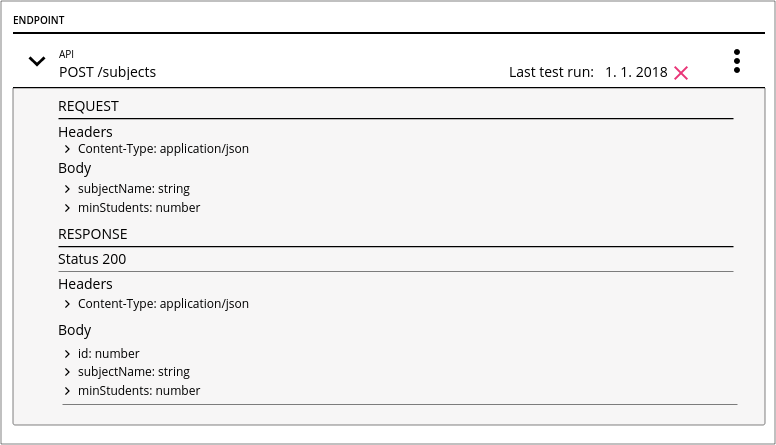
\includegraphics[scale=0.4]{./designs/drafts-1.0/api-detail.png}
	\caption{A~leaf node of~a~hierarchical structure that is used for~displaying
	the~information about~API's endpoints.}
	\label{api-detail}
\end{figure}

\section{Creating the~Test Case}
Even though it is important to~present the~API's endpoints to~the~users
in~a~friendly way, the~main focus of~the~application lies in~the~test cases.
For~that particular reason the~Test Case Creator was designed. The~design is
based on~canvas, which is a~HTML~5 element that allows for~dynamic, scriptable
rendering of~2D shapes and~bitmap images. The~Creator is designed as~an~dynamic
editor that allows users to~build test cases using various endpoints, test cases
and~control structures. The~idea behind it is that the~users will be able
to~construct complex test cases in~the~same way as~they would create state
machine diagrams\footnote{A~state machine diagram is a~behavior diagram which
showsh discrete behavior of~a~part of~designed system through finite state
transitions.}.

\begin{figure}[!hbt]
	\centering
	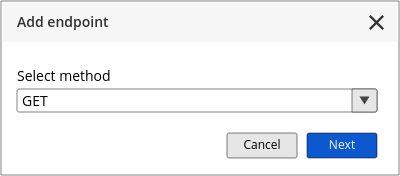
\includegraphics[scale=0.4]{./designs/drafts-1.0/add-endpoint-1.png}
	\caption{A~modal window for adding endpoint to~a~test case -- selecting
	the~endpoint's HTTP method.}
	\label{add-endpoint-1}
\end{figure}

The~Creator consists of~several parts. All of~them together allows users
to~model desired test cases using the~drag and~drop functionality. To~clarify,
consider an~example shown in~the~figure~\ref{test-case-creator}. In~the~example,
using the~drag and~drop functionality was inserted several endpoints
to~the~canvas. When an~endpoint is dropped to~the~canvas a~modal window with
endpoint's settings appears. If the~dropped endpoint was not a~leaf node
the~modal window asks the~user to~select endpoint's method
as~shown~in~the~figure~\ref{add-endpoint-1}.

\begin{figure}[!hbt]
	\centering
	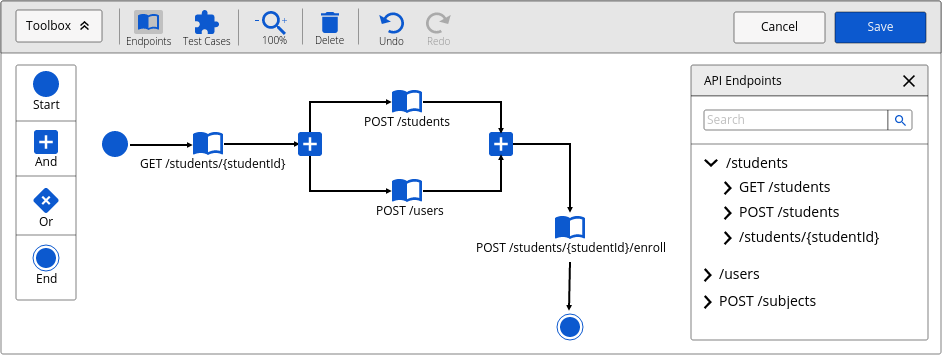
\includegraphics[scale=0.4]{./designs/drafts-1.0/test-case-creator.png}
	\caption{The~Test Case Creator with an~example of~a~test case in~the~format
	of~as~state machine diagram.}
	\label{test-case-creator}
\end{figure}

However, if the~endpoint was a~leaf node the~modal window with endpoint's detail
is shown as~can be seen in~the~figure~\ref{add-endpoint-2}. Then either
the~endpoint's details can be filled using the~form in~the~modal or~skipping
the~form and~using another endpoint's output as~the~endpoint's details -- simply
connecting them in~the~canvas. Overall, the~figure~\ref{test-case-creator} is
modelling simple test case that will find a~student by~given id, uses its
information details as~an~input for~creating new student and~a~user, and~tehn
enrolling the~newly created student to~some~course.

\begin{figure}[!hbt]
	\centering
	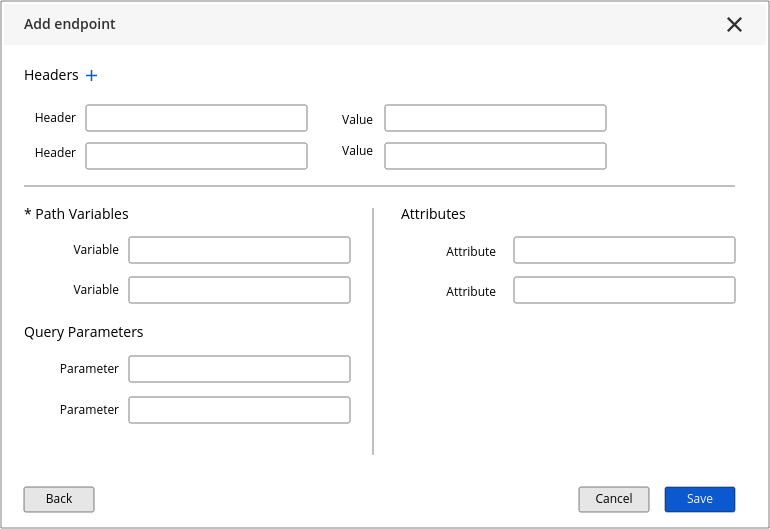
\includegraphics[scale=0.4]{./designs/drafts-1.0/add-endpoint-2.png}
	\caption{A~modal window for adding endpoint to~a~test case -- filling
	the~endpoint's information.}
	\label{add-endpoint-2}
\end{figure}

Once the~test case is creates using the~Creator, the~users should be allow
to~view, edit, and~run it. Hence the~Test Cases Overview was designed. As~can be
seen in~the~figure~\ref{test-cases}, the~overview consists of~a~navigation bar
with~buttons that allow managing the~test cases, e.g. creating, running
or~removing them. Following the~design, the~table with~test cases was created.
The~table allows users to~view, sort and~filter all test cases in~the~project.
Each test case in~the~table consists of~basic information about it, such
as~the~day when it was last run or~whether the~last run was successful or~not.
The~name of~the~test case in~the~table is then~used to~create a~link that
enables users to~edit the~test case in~the~Creator.

\begin{figure}[!hbt]
	\centering
	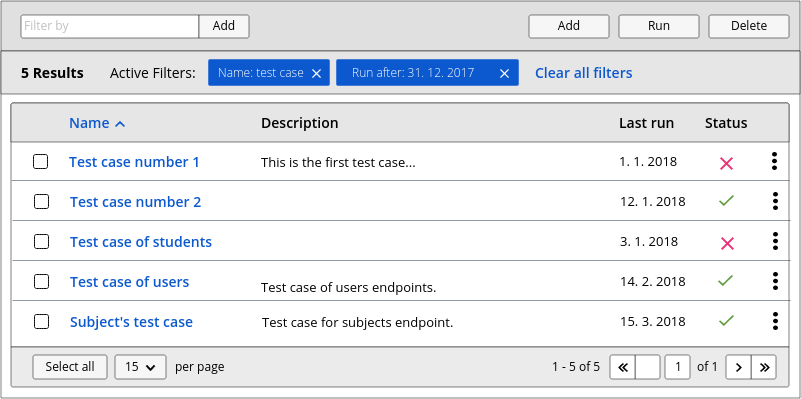
\includegraphics[scale=0.4]{./designs/drafts-1.0/test-cases.png}
	\caption{The~Test Cases Overview that contains information about created test
	cases.}
	\label{test-cases}
\end{figure}

% ===============================================================================



\chapter{Implementation and Testing}
zminit se o zmene dashboardu z rychleho prepinani projektu na breadcrumbs


\chapter{Conclusion}
The~aim of~this term project was to~design an~application that will allow its
users to~create test cases from~other applications API. As~a~part of~working
on~the~above goal the~technologies and~frameworks that will be needed when
building the~application upon~the~design were presented.

On~top of~that using patterns from~the~PatternFly framework the~first
application's designs were created and~the~most important part
of~the~application -- the~Test Case Creator was designed as~an~interactive
editor that uses simplified state machine diagrams to~allow users to~build the~test
cases easily and~fastly.

For~the~future, the~following improvements are planned such as~redesign of~the
endpoint's details that would allow the~users to~fill in~some~default data
for~that particular endpoint, which would allow the~users to~add endpoints
directly to~the~test cases without the~need to~specify the~endpoint's data.

Another key step is to~implement the~application using the~technologies listed
in~Chapter~\ref{Technologies} and~to~test it~using the~Red Hat JBoss BPM Suite
as~a~test project.

% TODO co by slo vylepsit 
% aby Test Case Creator umel i cykly a slozky pro test casy

%https://blog.readme.io/what-is-swagger-and-why-it-matters/

%================================================================================
 % viz. obsah.tex / see obsah.tex

  % Pouzita literatura / Bibliography
  % ----------------------------------------------
\ifslovak
  \makeatletter
  \def\@openbib@code{\addcontentsline{toc}{chapter}{Literatúra}}
  \makeatother
  \bibliographystyle{bib-styles/czechiso}
\else
  \ifczech
    \makeatletter
    \def\@openbib@code{\addcontentsline{toc}{chapter}{Literatura}}
    \makeatother
    \bibliographystyle{bib-styles/czechiso}
  \else 
    \makeatletter
    \def\@openbib@code{\addcontentsline{toc}{chapter}{Bibliography}}
    \makeatother
    \bibliographystyle{bib-styles/englishiso}
  %  \bibliographystyle{alpha}
  \fi
\fi
  \begin{flushleft}
  \bibliography{projekt-20-literatura-bibliography}
  \end{flushleft}

  % vynechani stranky v oboustrannem rezimu
  % Skip the page in the two-sided mode
  \iftwoside
    \cleardoublepage
  \fi

  % Prilohy / Appendices
  % ---------------------------------------------
  \appendix
\ifczech
  \renewcommand{\appendixpagename}{Přílohy}
  \renewcommand{\appendixtocname}{Přílohy}
  \renewcommand{\appendixname}{Příloha}
\fi
\ifslovak
  \renewcommand{\appendixpagename}{Prílohy}
  \renewcommand{\appendixtocname}{Prílohy}
  \renewcommand{\appendixname}{Príloha}
\fi
%  \appendixpage

% vynechani stranky v oboustrannem rezimu
% Skip the page in the two-sided mode
%\iftwoside
%  \cleardoublepage
%\fi
  
\ifslovak
%  \section*{Zoznam príloh}
%  \addcontentsline{toc}{section}{Zoznam príloh}
\else
  \ifczech
%    \section*{Seznam příloh}
%    \addcontentsline{toc}{section}{Seznam příloh}
  \else
%    \section*{List of Appendices}
%    \addcontentsline{toc}{section}{List of Appendices}
  \fi
\fi
  \startcontents[chapters]
  \setlength{\parskip}{0pt}
  % seznam příloh / list of appendices
  % \printcontents[chapters]{l}{0}{\setcounter{tocdepth}{2}}
  
  \ifODSAZ
    \setlength{\parskip}{0.5\bigskipamount}
  \else
    \setlength{\parskip}{0pt}
  \fi
  
  % vynechani stranky v oboustrannem rezimu
  \iftwoside
    \cleardoublepage
  \fi
  % Tento soubor nahraďte vlastním souborem s přílohami (nadpisy níže jsou pouze pro příklad)
% This file should be replaced with your file with an appendices (headings below are examples only)

% Umístění obsahu paměťového média do příloh je vhodné konzultovat s vedoucím
% Placing of table of contents of the memory media here should be consulted with a supervisor
%\chapter{Obsah přiloženého paměťového média}

%\chapter{Manuál}

%\chapter{Konfigurační soubor} % Configuration file

%\chapter{RelaxNG Schéma konfiguračního souboru} % Scheme of RelaxNG configuration file

%\chapter{Plakát} % poster
 % viz. prilohy.tex / see prilohy.tex
\end{document}
